
%\title{Error Correction in a Phenomenological Fibonacci Anyon Quantum Code}
\title{Random Fibonacci Anyons Simulable via Covariant Action of Mapping Class Group}

\author{Simon Burton, Courtney Brell, Steven Flammia}
%\date{\today}

\documentclass[12pt,a4paper]{article}
%\documentclass[11pt, twocolumn]{article}

\usepackage[paper=a4paper,dvips,top=1.5cm,left=1.5cm,right=1.5cm,
    foot=1cm,bottom=1.5cm]{geometry}

%\usepackage{epsf}
\usepackage{amsmath}
\usepackage{color}
\usepackage{natbib}
%\usepackage{cite}

\RequirePackage{amsmath}
\RequirePackage{amssymb}
\RequirePackage{amsthm}
%\RequirePackage{algorithmic}
%\RequirePackage{algorithm}
%\RequirePackage{theorem}
%\RequirePackage{eucal}
\RequirePackage{color}
\RequirePackage{url}
\RequirePackage{mdwlist}

\RequirePackage[all]{xy}
\CompileMatrices
\RequirePackage{hyperref}
\RequirePackage{graphicx}
\RequirePackage[dvips]{geometry}


\begin{document}

\maketitle

\def\Complex {C}
\def\tensor{\otimes}
\def\Tensor{\bigotimes}
\def\bra #1{\langle #1|}
\def\ket #1{|#1\rangle}
\def\braket #1#2{\langle #1|#2 \rangle}

%\def\Set{\widetilde{\text{Set}}}
%\def\Top{\widetilde{\text{Top}}}
%\def\Vec{\widetilde{\text{Vec}}}
%\def\Chain{\widetilde{\text{Chain}}}

%\def\ker{\text{ker}}
%\def\coker{\text{coker}}
%\def\im{\text{im}}

%\def\H{\mathcal{H}}
%\def\H{H}
%\def\S{S}
\def\mathZ{\mathbb{Z}}
\def\mathR{\mathbb{R}}

%\def\nin{\not\in}

%\def\heading #1{\noindent\underline{\Large\bf #1}}
\def\heading #1{\vskip 20pt \noindent\underline{\large \bf #1}\vskip 5pt}

\def\important #1{\underline{\bf #1}}

% ----------------------------------------------------------------------------
%

\heading{Braid group}

Braid group on $n$ strands is the group $B_n$ generated by $n-1$ generators
$\sigma_1, \sigma_2, ... \sigma_{n-1}$ with the following relations:
    $$ \sigma_i \sigma_j = \sigma_j \sigma_i \ \text{when}\ |i-j| > 2, $$
    $$ \sigma_i \sigma_{i+1} \sigma_i =  \sigma_{i+1} \sigma_i \sigma_{i+1}.$$


% ----------------------------------------------------------------------------

\heading{Fibonacci Anyons}


So we have a (linear) representation of the braid group:

    $$ \kappa : B_n \to GL(F_n).$$

Where $F_n$ is the Hilbert state space of $n$ Fibonacci anyons with
trivial total charge.


% ----------------------------------------------------------------------------

\heading{Curve Diagrams}

The disc $D = \{ x\in \mathR^2\ s.t.\ |x|\leq 1 \} $,
has boundary $\partial D = \{ x\in \mathR^2\ s.t.\ |x|=1 \} $.

Given a finite set $ Q_n \subset D-\partial D$,
we denote $D_n$ as the pair $(D, Q_n).$
%Topologically, this definition does not depend on
%anything but the cardinality of $Q_n.$

We define the mapping class group of $D_n$,
$MCG(D_n),$ as the set of homeomorphisms $D\to D$ that
restrict to a permutation on $Q_n,$ modulo isotopy that
fixes $Q_n.$
Such an equivelance class
of homeomorphisms will be denoted as $\phi:D_n\to D_n.$

We can think of $D_n$ as the unit disc with $n$ holes,
and the mapping class group as the set of homeomorphisms on
this space, modulo isotopy.

The line $L = \{ x\in \mathR\ s.t.\ |x|\leq 1 \} $,
and a finite set $R_n\subset L$,
$L_n = (L, R_n).$

We define a curve diagram as an embedding $f : L\to D$ that
restricts to an injection $R_n\to Q_n,$ modulo
isotopy.
This will be denoted as $f : L_n\to D_n.$
We can generalize this to $f : L_m\to D_n$ with $m\leq n$
to mean a map $L\to D$ that restricts to an injection $R_m\to Q_n,$
modulo isotopy.

DIAGRAM

% ----------------------------------------------------------------------------

\heading{Group action}

The mapping class group $MCG(D_n)$ acts on curve diagrams $f : L_n\to D_n$
via post-composition.

\important{Definition:} by a {\it local action} on a curve
diagram $f:L_n\to D_n$ we mean an element of $MCG(D_n)$
that can be represented by a half-twist that acts
on a small neighbourhood of $f([i, i+1]).$
We denote such an element by $b(i, f).$

\important{Definition:} by a {\it sequence of local moves} on a curve
diagram $f:L_n\to D_n$ we mean a
sequence of curve diagrams $f_k: L_n\to D_n$ and local actions:

        $$ b(i_1, f_1),\ b(i_2, f_2),\ ...\ b(i_N, f_N) $$

such that $f_1=f,$ and

        $$ f_{k+1} = b(i_k, f_k) f_k,\ \  \text{} 1\leq k<N.$$


% ----------------------------------------------------------------------------

\heading{Local factorization of $MCG(D_n)$}

\important{Problem:}
Given curve diagrams $f:L_n\to D_n$ and $g:L_2\to D_n$
find $\phi\in MCG(D_n)$ as a product of
a sequence of local moves such that % DIAGRAM
$g = \phi f i.$

\important{Solution:}

1) decompose $f$ along (finitely many) intersections
with $g.$

% DIAGRAM

2) on each component $k$:

% DIAGRAM

let $h_k = g_k + f_k.$
This is a simple closed curve in $D$ which splits $D$
into two regions, the inside (simply connected) and the
outside.
We find six cases, which we can distinguish between
using the winding number and whether the end points
of $f$ are inside or outside:

% DIAGRAM


% ----------------------------------------------------------------------------

\heading{Combinatorial formulation}

We discretize the prolem for software implementation...

% ----------------------------------------------------------------------------

\heading{Numerical results}

% ----------------------------------------------------------------------------

%Given a topological space $X$ we define the {\it mapping class group} of $X$ as
%the set of homeomorphisms $f:X\to X$ modulo isotopy
%
%    % $$ MCG(X) := \{ f : X \to X \text{s.t.} f \text{is homeomorphism} \} / \sim_{\text{iso}} $$
%    $$ MCG(X) := \{ f : X \to X \} / \sim_{\text{iso}}.$$

%Given a topological manifold $M$ we define the {\it mapping class group} of $M$ as
%the set of homeomorphisms $f:M\to M$ modulo isotopy
%
%    $$ MCG(M) := \{ f : M \to M \} / \sim_{\text{iso}}.$$
%
%If $M$ has boundary $\partial M$ we require the homeomorphisms to
%be the identity on $\partial M$.
%
%In particular we are interested in
% the $n$-punctured disc.
%This is a disc $D = \{ x\in \mathR^2 s.t. |x|\leq 1 \} $
%with $n$ points removed:
%
%    $$ D_n := D - Q_n,$$
%
%where $Q_n$ is some finite subset of the interior of $D$.
%
%%topologically this is a sphere with $n+1$ holes in it.
%
%It is a theorem that the group $MCG(D_n)$ is isomorphic to $B_n.$
%(See \cite{Kassel10}, chapter 1.)
%
%We fix $Q_n$ to be the points $\{(0, i/(n+1)) for i=1,...n\}$
%then we define the line $L = \{(0, x) s.t. |x|\leq 1\}.$
%Given a representative $f$ of an element of $MCG(D_n)$
%we define the
%curve diagram as the
%image of $L$ under $f$.
%
%It is a theorem (see \cite{Dehornoy02}) that such curve diagrams
%correspond uniquely to elements of the mapping class group, and
%hence to the braid group $B_n$.



\heading{Braid group representation}


Here we verify the braid relations directly:

\begin{center}
%\includegraphics[width=0.5\textwidth]{mypicture.png}
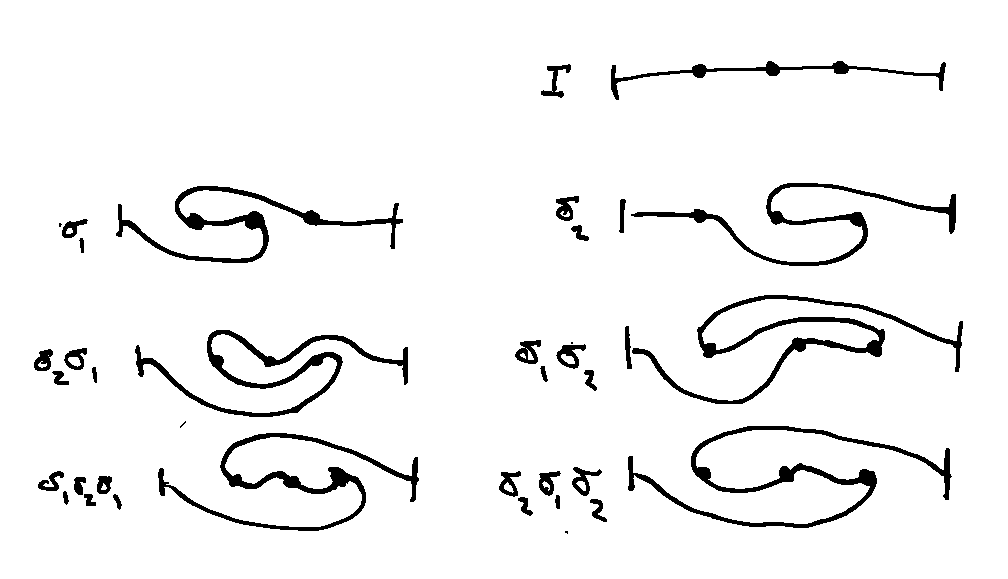
\includegraphics[width=0.5\textwidth]{curve-braid.eps}
\end{center}

\cite{Dehornoy02}


% ----------------------------------------------------------------------------

%\heading{Pair-of-pants decompositions}

%We measure charge in regions bounded by curves, ie. elements of
%the first homology group $H_1(D_n).$


%http://arxiv.org/pdf/1002.2816.pdf
%http://www.math.ucsb.edu/~zhenghwa/data/course/lecture_notes/Chap2.pdf
%http://physics.stackexchange.com/questions/93183/about-the-atiyah-segal-axioms-on-topological-quantum-field-theory
%http://mathoverflow.net/questions/359/a-reading-list-for-topological-quantum-field-theory
%http://projecteuclid.org/download/pdf_1/euclid.cmp/1104178138
%http://arxiv.org/pdf/math/9912085v1.pdf


% ----------------------------------------------------------------------------

\bibliography{refs}{}
\bibliographystyle{abbrv}

\end{document}


